% Observed values are generated from published-contrasts.json; no new model runs.
\begin{figure*}[t]
\centering
\begingroup
\definecolor{ragink}{HTML}{252A30}
\definecolor{ragmuted}{HTML}{68717A}
\definecolor{ragrule}{HTML}{D8DDE1}
\definecolor{ragblue}{HTML}{526F89}
\definecolor{ragpurple}{HTML}{7B7088}
\definecolor{ragsage}{HTML}{5C7B6E}
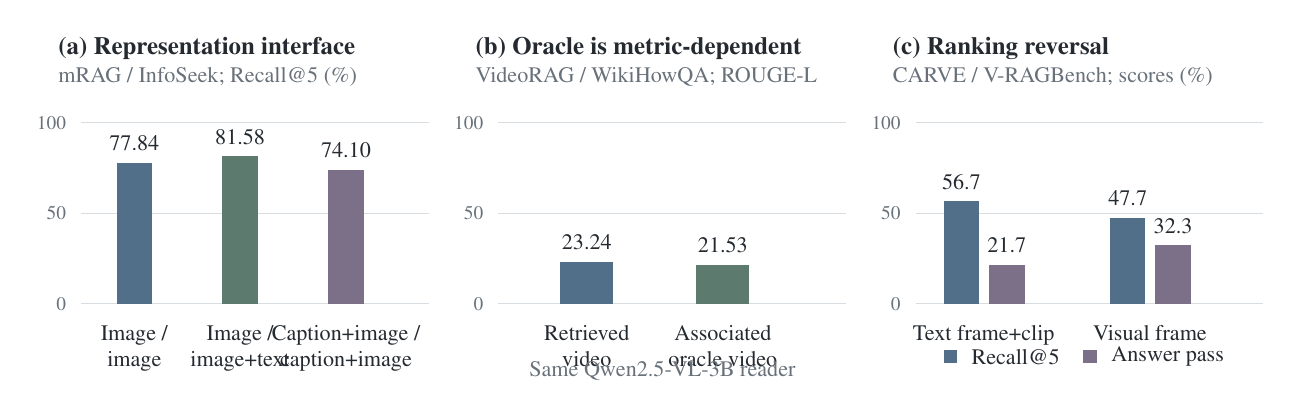
\begin{tikzpicture}[x=.96cm,y=1cm,font=\fontsize{8}{9.4}\fontfamily{ptm}\selectfont,text=ragink]
\begin{scope}[xshift=0cm]
\node[anchor=west,font=\fontsize{9}{10}\fontfamily{ptm}\bfseries] at (0,3.8) {(a) Representation interface};
\node[anchor=west,text=ragmuted] at (0,3.43) {mRAG / InfoSeek; Recall@5 (\%)};
\draw[ragrule,line width=.35pt] (.43,0.55) -- (5.03,0.55);\node[anchor=east,text=ragmuted,font=\fontsize{7}{8}\fontfamily{ptm}\selectfont] at (.36,0.55) {0};
\draw[ragrule,line width=.35pt] (.43,1.7) -- (5.03,1.7);\node[anchor=east,text=ragmuted,font=\fontsize{7}{8}\fontfamily{ptm}\selectfont] at (.36,1.7) {50};
\draw[ragrule,line width=.35pt] (.43,2.8499999999999996) -- (5.03,2.8499999999999996);\node[anchor=east,text=ragmuted,font=\fontsize{7}{8}\fontfamily{ptm}\selectfont] at (.36,2.8499999999999996) {100};
\fill[ragblue] (0.90,0.55) rectangle (1.37,2.340);\node[anchor=south] at (1.135,2.365) {77.84};\node[align=center,anchor=north] at (1.135,.40) {Image /\\image};
\fill[ragsage] (2.30,0.55) rectangle (2.77,2.426);\node[anchor=south] at (2.535,2.451) {81.58};\node[align=center,anchor=north] at (2.5349999999999997,.40) {Image /\\image+text};
\fill[ragpurple] (3.70,0.55) rectangle (4.17,2.254);\node[anchor=south] at (3.935,2.279) {74.10};\node[align=center,anchor=north] at (3.935,.40) {Caption+image /\\caption+image};
\end{scope}
\begin{scope}[xshift=5.3cm]
\node[anchor=west,font=\fontsize{9}{10}\fontfamily{ptm}\bfseries] at (0,3.8) {(b) Oracle is metric-dependent};
\node[anchor=west,text=ragmuted] at (0,3.43) {VideoRAG / WikiHowQA; ROUGE-L};
\draw[ragrule,line width=.35pt] (.43,.55) -- (5.03,.55);\node[anchor=east,text=ragmuted,font=\fontsize{7}{8}\fontfamily{ptm}\selectfont] at (.36,.55) {0};
\draw[ragrule,line width=.35pt] (.43,1.70) -- (5.03,1.70);\node[anchor=east,text=ragmuted,font=\fontsize{7}{8}\fontfamily{ptm}\selectfont] at (.36,1.70) {50};
\draw[ragrule,line width=.35pt] (.43,2.85) -- (5.03,2.85);\node[anchor=east,text=ragmuted,font=\fontsize{7}{8}\fontfamily{ptm}\selectfont] at (.36,2.85) {100};
\fill[ragblue] (1.25,.55) rectangle (1.95,1.08452);\node[anchor=south] at (1.60,1.11) {23.24};
\fill[ragsage] (3.05,.55) rectangle (3.75,1.04519);\node[anchor=south] at (3.40,1.075) {21.53};
\node[anchor=north,align=center] at (1.60,.40) {Retrieved\\video};
\node[anchor=north,align=center] at (3.40,.40) {Associated\\oracle video};
\node[text=ragmuted] at (2.60,-.30) {Same Qwen2.5-VL-3B reader};
\end{scope}
\begin{scope}[xshift=10.6cm]
\node[anchor=west,font=\fontsize{9}{10}\fontfamily{ptm}\bfseries] at (0,3.8) {(c) Ranking reversal};
\node[anchor=west,text=ragmuted] at (0,3.43) {CARVE / V-RAGBench; scores (\%)};
\draw[ragrule,line width=.35pt] (.43,0.55) -- (5.03,0.55);\node[anchor=east,text=ragmuted,font=\fontsize{7}{8}\fontfamily{ptm}\selectfont] at (.36,0.55) {0};
\draw[ragrule,line width=.35pt] (.43,1.7) -- (5.03,1.7);\node[anchor=east,text=ragmuted,font=\fontsize{7}{8}\fontfamily{ptm}\selectfont] at (.36,1.7) {50};
\draw[ragrule,line width=.35pt] (.43,2.8499999999999996) -- (5.03,2.8499999999999996);\node[anchor=east,text=ragmuted,font=\fontsize{7}{8}\fontfamily{ptm}\selectfont] at (.36,2.8499999999999996) {100};
\fill[ragblue] (0.80,0.55) rectangle (1.27,1.854);\node[anchor=south] at (1.035,1.879) {56.7};
\fill[ragpurple] (1.40,0.55) rectangle (1.87,1.049);\node[anchor=south] at (1.635,1.074) {21.7};
\fill[ragblue] (3.00,0.55) rectangle (3.47,1.647);\node[anchor=south] at (3.235,1.672) {47.7};
\fill[ragpurple] (3.60,0.55) rectangle (4.07,1.293);\node[anchor=south] at (3.835,1.318) {32.3};
\node[anchor=north] at (1.33,.40) {Text frame+clip};\node[anchor=north] at (3.53,.40) {Visual frame};
\fill[ragblue] (.8,-.2) rectangle (.98,-.04);\node[anchor=west] at (1.04,-.12) {Recall@5};\fill[ragpurple] (2.65,-.2) rectangle (2.83,-.04);\node[anchor=west] at (2.89,-.12) {Answer pass};
\end{scope}
\end{tikzpicture}
\endgroup
\caption{Published counterexamples to monotonic improvement. (a) Where a representation is added matters~\citep[Table~3]{arxiv250524073}. (b) The associated oracle video does not maximize this reader's ROUGE-L; the same paper's G-Eval moves in the opposite direction~\citep[Table~1]{jeong2025videorag}. (c) Retrieval and answer rankings can reverse when representations change~\citep[Table~3]{lee2026carve}. Panels retain distinct protocols; Appendix~\ref{app:published-contrasts} records versions, corpora, readers, and limits.}
\label{fig:audited-contrasts}
\end{figure*}
